\documentclass[border=7pt]{standalone}
\usepackage{tikz}
\begin{document}
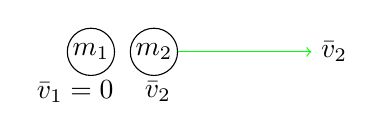
\begin{tikzpicture}
  \draw (4.4,0) circle [radius=0.3]  node {$m_1$};
  \draw (5.2,0) circle [radius=0.3]  node {$m_2$};
  \node (c) at (4.2,-0.5){$\bar{v}_1=0$};
  \node (c) at (5.25,-0.5){$\bar{v}_2$};
  \draw [green, ->] (5.5,0) -- (7.2,0) node [black, right] {$\bar{v}_2$};
\end{tikzpicture}
\end{document}
